\documentclass[11pt]{article}

\usepackage{amsfonts}
%\usepackage{geometry}
\usepackage[paper=a4paper, 
            left=20.0mm, right=20.0mm, 
            top=25.0mm, bottom=25.0mm]{geometry}
\pagestyle{empty}
\usepackage{graphicx}
\usepackage{fancyhdr, lastpage, bbding, pmboxdraw}
\usepackage[usenames,dvipsnames]{color}
\definecolor{darkblue}{rgb}{0,0,.6}
\definecolor{darkred}{rgb}{.7,0,0}
\definecolor{darkgreen}{rgb}{0,.6,0}
\definecolor{red}{rgb}{.98,0,0}
\usepackage[colorlinks,pagebackref,pdfusetitle,urlcolor=darkblue,citecolor=darkblue,linkcolor=darkred,bookmarksnumbered,plainpages=false]{hyperref}
\renewcommand{\thefootnote}{\fnsymbol{footnote}}

\pagestyle{fancyplain}
\fancyhf{}
\lhead{ \fancyplain{}{Course Name} }
%\chead{ \fancyplain{}{} }
\rhead{ \fancyplain{}{\today} }
%\rfoot{\fancyplain{}{page \thepage\ of \pageref{LastPage}}}
\fancyfoot[RO, LE] {Page \thepage\ of \textcolor{black}{\pageref{LastPage}} }
\thispagestyle{plain}

%%%%%%%%%%%% LISTING %%%
\usepackage{listings}
\usepackage{caption}
\usepackage{subcaption}
\DeclareCaptionFont{white}{\color{white}}
\DeclareCaptionFormat{listing}{\colorbox{gray}{\parbox{\textwidth}{#1#2#3}}}
\captionsetup[lstlisting]{format=listing,labelfont=white,textfont=white}
\usepackage{verbatim} % used to display code
\usepackage{fancyvrb}
\usepackage{acronym}
\usepackage{amsthm, amsmath}
\usepackage{tikz}
    \usetikzlibrary{calc, arrows, arrows.meta, positioning}
\usepackage{amssymb,amsmath,stackengine}
\stackMath
\usepackage{ifthen}

\VerbatimFootnotes % Required, otherwise verbatim does not work in footnotes!

\definecolor{OliveGreen}{cmyk}{0.64,0,0.95,0.40}
\definecolor{CadetBlue}{cmyk}{0.62,0.57,0.23,0}
\definecolor{lightlightgray}{gray}{0.93}

\lstset{
	%language=bash,                          % Code langugage
	basicstyle=\ttfamily,                   % Code font, Examples: \footnotesize, \ttfamily
	keywordstyle=\color{OliveGreen},        % Keywords font ('*' = uppercase)
	commentstyle=\color{gray},              % Comments font
	numbers=left,                           % Line nums position
	numberstyle=\tiny,                      % Line-numbers fonts
	stepnumber=1,                           % Step between two line-numbers
	numbersep=5pt,                          % How far are line-numbers from code
	backgroundcolor=\color{lightlightgray}, % Choose background color
	frame=none,                             % A frame around the code
	tabsize=2,                              % Default tab size
	captionpos=t,                           % Caption-position = bottom
	breaklines=true,                        % Automatic line breaking?
	breakatwhitespace=false,                % Automatic breaks only at whitespace?
	showspaces=false,                       % Dont make spaces visible
	showtabs=false,                         % Dont make tabls visible
	columns=flexible,                       % Column format
	morekeywords={__global__, __device__},  % CUDA specific keywords
}

\newcommand{\question}[1]{\section*{\normalsize #1}}
% \newcommand{\mat}[1]{\begin{bmatrix}#1\end{bmatrix}}
% \newcommand{\extraspace}[]{
%     \begin{center}
%         \textbf{Use this page for extra space.}
%     \end{center}
% }


\DeclareMathOperator*{\argmax}{arg\,max}
\DeclareMathOperator*{\argmin}{arg\,min}
%\DeclareMathOperator*{\vec}[1]{\textbf{#1}}

\newcommand{\squig}{{\scriptstyle\sim\mkern-3.9mu}}
\newcommand{\lsquigend}{{\scriptstyle\lhd\mkern-3mu}}
\newcommand{\rsquigend}{{\scriptstyle\rule{.1ex}{0ex}\rhd}}
\newcounter{sqindex}
\newcommand\squigs[1]{%
  \setcounter{sqindex}{0}%
  \whiledo {\value{sqindex}< #1}{\addtocounter{sqindex}{1}\squig}%
}
\newcommand\rsquigarrow[2]{%
  \mathbin{\stackon[2pt]{\squigs{#2}\rsquigend}{\scriptscriptstyle\text{#1\,}}}%
}
\newcommand\lsquigarrow[2]{%
  \mathbin{\stackon[2pt]{\lsquigend\squigs{#2}}{\scriptscriptstyle\text{\,#1}}}%
}


\begin{document}
\begin{center}
    {\Large \textsc{Written Assignment 1}}
\end{center}
\begin{center}
    Due: Friday 02/02/2024 @ 11:59pm EST
\end{center}

\section*{\textbf{Disclaimer}}
I encourage you to work together, I am a firm believer that we are at our best (and learn better) when we communicate with our peers. Perspective is incredibly important when it comes to solving problems, and sometimes it takes talking to other humans (or rubber ducks in the case of programmers) to gain a perspective we normally would not be able to achieve on our own. The only thing I ask is that you report who you work with: this is \textbf{not} to punish anyone, but instead will help me figure out what topics I need to spend extra time on/who to help. When you turn in your solution (please use some form of typesetting: do \textbf{NOT} turn in handwritten solutions), please note who you worked with.\newline

\noindent Remember that if you have a partner, you and your partner should submit only \textbf{one} submission on gradescope.



\question{Question 1: Shortest Path Composition (25 points)}
Consider a graph $G = (V, E, w: E\rightarrow \mathbb{R}^{\ge 0})$ where $V$ is a set of vertices, $E$ is a set of (directed) edges, and $w$ is a \textit{weight function} that maps edges to weights where each weight is $\ge 0$. Let us define a path $p$ to be a sequence of edges where the destination vertex of one edge is the source vertex of the next edge (if the next edge exists). Let us define the \textit{cost} of an path the traditional way, i.e. the cost of a path $p$ is the sum of the edge weights in $p$:
$$cost(p) = \sum\limits_{e\in p} w(e)$$
Show that if we know a shortest path $p^* = a\rsquigarrow{x}{4}b$ from vertex $a$ to vertex $b$ has cost $x$. If we know $p^*$ passes through intermediary vertex $c$, then let $p_1 = a\rsquigarrow{y}{4}c$, and let $p_2 = c\rsquigarrow{z}{4}b$. Show that if $p^* = p_1 \cup p_2$, then $p_1$ is a shortest path from $a$ to $c$, and that $p_2$ is a shortest path from $c$ to $b$.

\medskip
\hrule
\medskip

If there was an edge that was in both $p_1$ and $p_2$, it would not be needed in $p_2$ because it would be going to a vertex that the path had already advanced to. (This wouldn't apply with negative weights, because cycling would give lesser costs, but we know the weights are nonnegative.) Therefore, $p_1 \cap p_2 = \emptyset$.

Now, since we also know $p^* = p_1 \cup p_2$ and they're disjoint, each path in $p^*$ is in either $p_1$ or $p_2$. Thus we may say $\sum_{e \in p^*} w(e) = \sum_{e_1 \in p_1} w(e_1) + \sum_{e_2 \in p_2} w(e_2)$. Looking back to our definitions this equation is the same as $x = y + z$.

For purposes of contradiction assume that $p_1$ is not the shortest path from $a$ to $c$. We can call the new cost of this path $y - k$, with $k > 0$. Then, revisiting our equation from before, if we use this new path, we have $x - k = y - k + z$ as the total cost. But then we've shown that it's possible to have a lower cost, so $p^*$ is not the shortest path. 

In either case, we reach an impossibility, so $p_1$ must be the shortest path from $a$ to $c$. We can use the exact same argument with $p_2$. 

\newpage

\question{Question 2: Best and Worst Cases for DFS (25 points)}
Consider a graph $G = (V, E, w: E\rightarrow \mathbb{R}^{\ge 0})$ where $V$ is a set of vertices, $E$ is a set of (directed) edges, and $w$ is a \textit{weight function} that maps edges to weights where each weight is $\ge 0$. Let us start a DFS search from vertex $a$, the goal of which is to find vertex $b$ (where $b\neq a$). In the worst case, where is the goal vertex $b$ in relation to the source vertex $a$ in the DFS expansion. How many vertices and edges must the expansion contain before when we reach $b$? What about the best case?

\medskip
\hrule
\medskip

\begin{enumerate}
    \item In the worst case the goal vertex would be at the very end of the DFS expansion. This could happen if the graph was a long chain with $a$ on one side and $b$ on the other.
    \item The expansion would have to have all $|V|$ vertices and all $|E|$ edges. The worst case would be a graph that looks like a long line, thus, there is a path from one end to another that has the cost of the sum of all edge-weights in the graph. If a certain edge $e$ were not included in the expansion, we would be subtracting the weight $w(e)$ from the total, which is guaranteed to be nonnegative, so this new path's cost would be less than or equal to our worst-case cost.
    \item The best case would occur if $a$ and $b$ were adjacent vertices with a directed edge from $a$ to $b$, and $a$ had only one outgoing edge or its outgoing edge to $b$ was the first one that we chose when conducting the search. That is, we'd have 2 vertices and 1 edge in our expansion. Note this is the best case as defined by the number of vertices and edges, not necessarily the total cost.
\end{enumerate}

\newpage

\question{Extra Credit: Heuristics for Pacman-NoGhosts (50 points)}
Consider a Pacman world with no ghosts, an example of which is shown below:

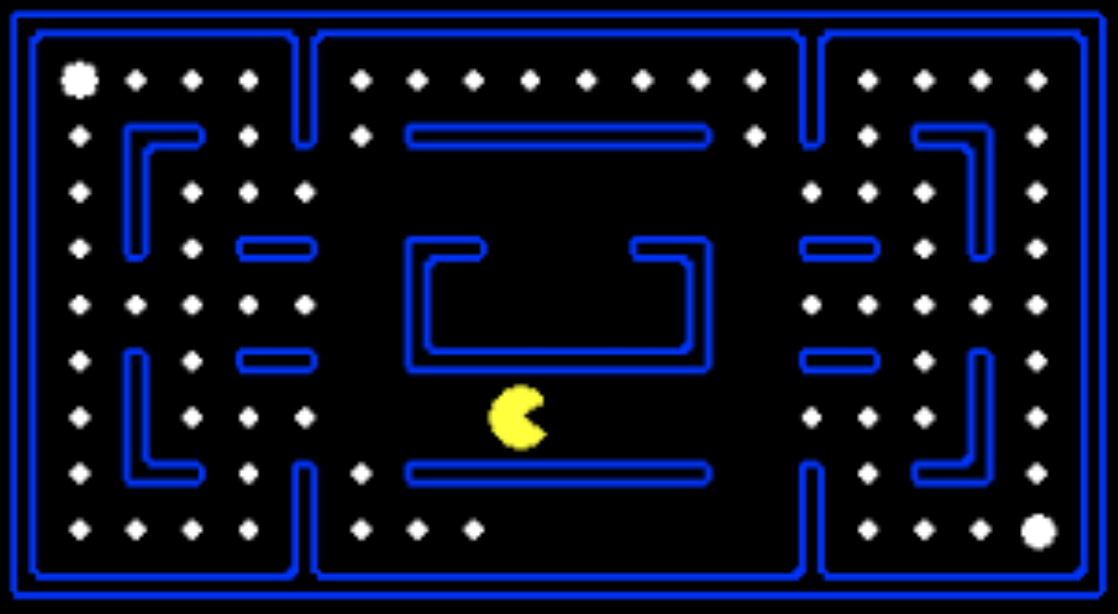
\includegraphics[width=0.8\linewidth]{./pacman-noghosts.png}

\noindent Here is the description of this search problem:
\begin{itemize}
    \item\textbf{Environment:} A 2-d map of finite size where each square can contain a wall, a food pellet, Pacman, or is unoccupied.
    \item\textbf{Sensors/State:} The state of the world is a structure containing the following fields (in Java-ish syntax):
        \begin{itemize}
            \item\texttt{current\_loc: Coordinate}: The (x,y) location of Pacman in the map.
            \item\texttt{food\_remaining\_locs: Collection<Coordinate>}: The (x,y) locations of all remaining food pellets in the map.
        \end{itemize}
    \item\textbf{Initial state:} The initial state is an instance of the State with the following field values:
        \begin{itemize}
            \item\texttt{current\_loc = (9, 3); // technically any unoccupied square will do}
            \item\texttt{food\_remaining\_locs = locations of all food pellets in the map; }
        \end{itemize}
    \item\textbf{Actuators/Actions:} Pacman can move to an adjacent square in a cardinal direction.
    \item\textbf{Transition Model:} Pacman will move to the adjacent square if it is not a wall and if the action will not take Pacman out of bounds of the map. Additionally, if Pacman enters a square that contains a food pellet, Pacman will automatically consume that pellet. When Pacman consumes a pellet, the location of that pellet is removed from the \texttt{food\_remaining\_locs} of that state.
    \item\textbf{Path cost:} Moving to an adjacent square has a cost of 1. Therefore, the cost of a path is the number of edges in the path.
    \item\textbf{Goal Test:} Any state where the number of remaining pellets is zero is a goal state regardless of the (x,y) position of Pacman.
    \item\textbf{Performance Measure:} The number of turns it takes to eat all of the food pellets.
\end{itemize}

\noindent In this problem, we want to minimize the performance metric (i.e. eat all of the pellets in the fewest number of turns). If we cast this problem into a search problem (where states are vertices and actions are edges), then we can use a search algorithm to find the shortest path from our initial state to a goal state. We will use the $A^*$ algorithm equipped with the goal-test function to do so.\newline

\noindent In order to use $A^*$, we need to define a heuristic that estimates the cost of the current state to a goal state. Design a heuristic that is admissible and consistent that will solve this problem. Your heuristic must be non-negative and must return 0 when the current state is a goal state.\newline\newline

\noindent\textit{Hint:} If we are at a square that contains a food pellet, then the smallest cost to a goal state is the number of movements to enter all of the squares that still contain food pellets. So, something we would like to know (and probably cache beforehand) are the distances between pairs of squares that contain food pellets.

\medskip
\hrule
\medskip

% Do it where you have pellets left + distance between closest pellet

One heuristic that we could use is the number of pellets remaing (from \texttt{food\_remaining\_locs.size()}) plus the Manhattan distance from Pacman to the closest food pellet minus 1. If there are no remaining food pellets the distance is considered 1 (The smallest it could be otherwise).

This heuristic is admissible and consistent because it will always overestimate, or be a perfect estimate of, the actual cost. Consider the case where Pacman is directly adjacent to all $n$ of the remaing pellets, which are contiguous. In that case the heuristic will estimate $n + (1 - 1) = n$, which is the actual remaing cost. If there are any gaps between pellets in the future (after Pacman has gobbled up the closest food pellet), the heuristic will pretend that the cost of doing so is 0, so we will always overestimate here.

However, it is still reasonable in that it \textit{will} incentivize Pacman to go towards nearby pellets and eat food when possible. Pacman will continue through groupings of pellets when possible, similar to how a human might play.

\end{document}

